\chapter{Results}
\label{capitulo5}

In this chapter, the results collected from the Chapter 4 will be discussed and analyzed. It is essential to freeze that only approach three from \ref{sub:3} was implemented into the framework because the goal was to work with multiple cameras and multi-view perspectives.

The algorithms and the simulations was performed in a computer with this follow configuration:

\begin{itemize}
    \item Operational System Ubuntu 18.04
    \item CPU Intel core i7 7700HQ 2.80 GHz
    \item 32 GB memory RAM
    \item GPU Nvidia Geforce GTX 1050 Ti - 4 GB
\end{itemize}


The framework can perform the tests on the Audi test track, as shown in Figure \ref{fig:test_track}, but in this work, only the proof of concept of the algorithms was performed. 

\begin{figure}[H]
\centering
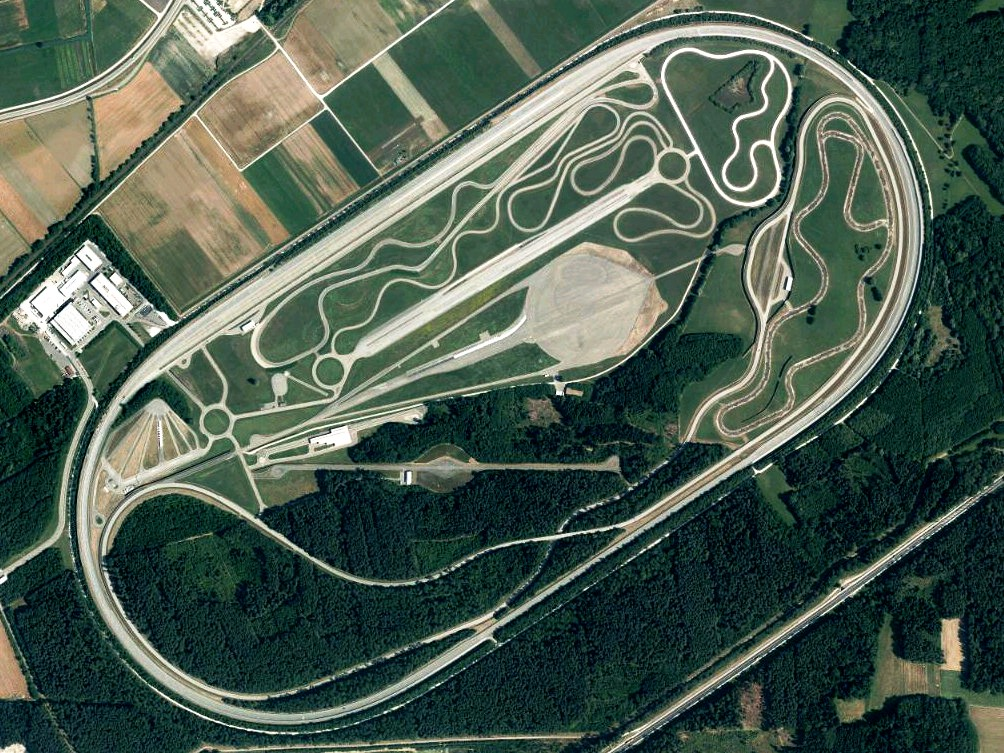
\includegraphics[scale=0.3]{imagens/testtrack.jpg}
\caption{Audi test track in eagle's view}
\label{fig:test_track}
\end{figure}


The algorithm for object detection was performed over the parking lot of the company EFS GmbH as shown in Figure \ref{fig:park}.


\begin{figure}[H]
\centering
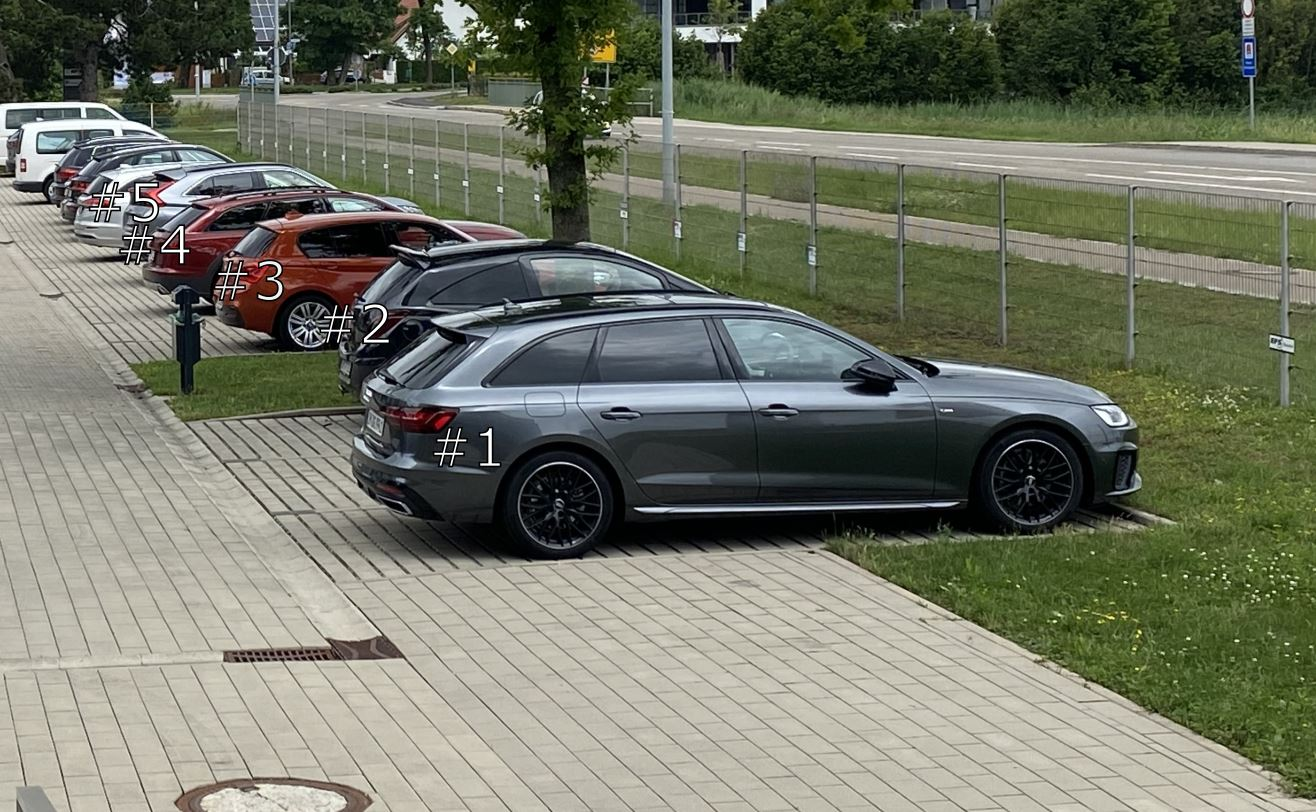
\includegraphics[scale=0.5]{imagens/park.JPG}
\caption{Position of the cars on the parking lot}
\label{fig:park}
\end{figure}

\section{Description of the test scenario}

The test scenario was built three times, using different perspectives. For the first test where it was necessary to use the camera, calibration perspective was made using only one camera, and the height of this camera does not matter to compute the distance, only a known distance, and dimensions of a known object to adjust this algorithm.

For the second scenario, some photos were taken and labeled with the known metrics to support the training step and return a useful result according to reality. 

The last approach and used in this work to built the framework was used following some principles as the cameras should be mounted at the same level, the same horizontal position,  the stream must be captured at the same time of the camera and sent to the same control center to process this data. 

The used cameras were GoPro 5, which allow building a wireless network with many cameras. 


\section{Results with camera calibration}

The results from approach one from \ref{sub:1} were implemented using Python 3.7 and Opencv3, and the position was computed based on camera calibration. Equation (\ref{eq:focal_distance}) is defined as the distance used in the camera calibration, using a measurer tape and a piece of paper ($21.59$ cm x  $27.94$ cm), and this was positioned $60.96$ cm in front of the camera to take the photo.

\begin{equation}
    \label{eq:focal_distance}
    F = \frac{P\cdot D}{W}
\end{equation}

W is the piece of the paper's width, which is $27.94$ cm, D is the distance from the piece of paper to the camera, and P is the paper's measure in pixels taken from the image. Applying the (\ref{eq:focal_distance}), the focal length (F) is $541.09$ pixels.





The results achieved with this technique is shown in Table \ref{tab:output_calibrate}. 

\begin{table}[H]
\centering
\caption{Measurements achieved with camera calibration algorithm}
\begin{tabular}{l|l} 
\toprule
Car &  Measurements      \\
\#1   & 4.05        \\
\#2   & 10.67       \\
\#3   & 15.52       \\
\#4   & 19.55       \\
\#5   & 20.08       \\
\bottomrule
\end{tabular}
\label{tab:output_calibrate}
\end{table} 



\section{Results with known map}
In this section is detailed the results of the proposal with a known map. This approach was performed using the neural network from \ref{sub:2} and the data provided by KITTI Dataset \cite{geiger2013vision}. It is essential to freeze. This approach was used only for the comparison method and not to be used on the final framework. 


The results collected in this section are beneficial, as several companies and other universities are releasing the dataset as open source. There is a need to understand image manipulation, and in some cases, data from LIDAR and Radar.

This test's main idea was to get the information from the object detection performed with the algorithm using the boundary boxes approach, collect this known information as input in the neural network, and predict a distance from the camera until the object. Where in Figure \ref{fig:output} is shown an example of the known KITTI dataset, it serves just as motivation for this work. The final results were not performed over this dataset. 

\begin{figure}[H]
\centering
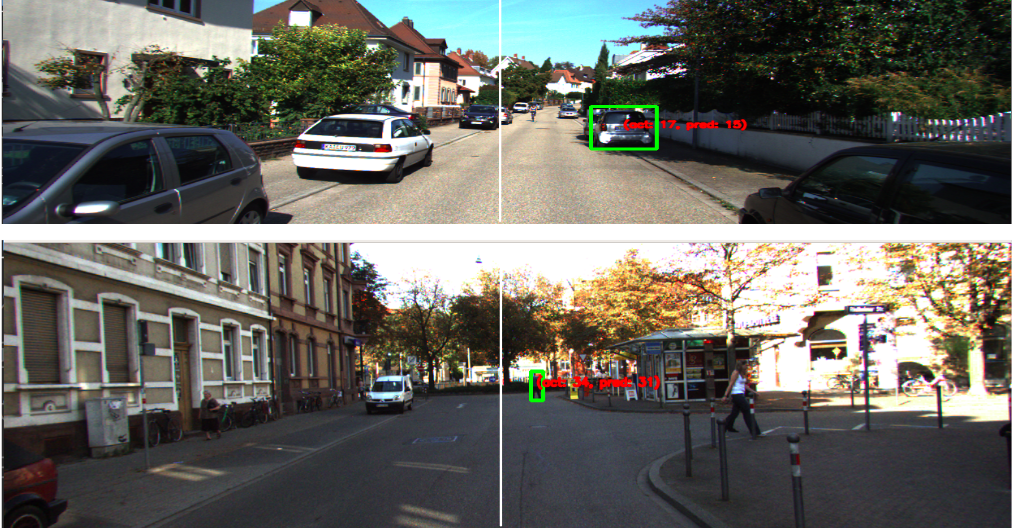
\includegraphics[width=\textwidth]{imagens/ouput.png}
\caption{Output results from framework using single stereo camera and known map}
\label{fig:output}
\end{figure}

For this approach, the output achieved from Table \ref{tab:output_table} was used for the first interaction and estimate the distance, as shown in Table \ref{tab:output_2}. These results are similar to the reality because it uses a known map, and the measurement step of these structures was performed and the labeling part.

\begin{table}[H]
\centering
\caption{Measurements achieved with camera and known map}
\begin{tabular}{l|l} 
\toprule
Car &  Measurements      \\
\#1   & 4.43        \\
\#2   & 10.98       \\
\#3   & 16.01       \\
\#4   & 18.99       \\
\#5   & 22.18       \\
\bottomrule
\end{tabular}
\label{tab:output_2}
\end{table} 


\section{Results with multi-cameras and proposed framework}


The proposed framework's algorithm predicts the objects of the whole scenario in 28 ms and has identified nine cars on the image, as shown in Figure \ref{fig:park_predict} and in Table \ref{tab:accuracy} is demonstrated the accuracy of each prediction for each vehicle. The output accuracies from the algorithm are shown in Table \ref{fig:framework_predict}. The low accuracies are related to the partially occluded objects, such as car two and car 6. 

The perspective of the distance this algorithm computed this using the Inverse Perspective Mapping (IPM) combined with the Yolo Algorithm, where the view of distance was fused on the last fully connected layer. In Table \ref{tab:output_framework} is shown the results achieved from the perspective using two cameras. 

\begin{table}[H]
\centering
\caption{Measurements achieved with multicameras}
\begin{tabular}{l|l} 
\toprule
Car &  Measurements      \\
\#1   & 4.40        \\
\#2   & 11.05       \\
\#3   & 16.01       \\
\#4   & 19.92       \\
\#5   & 24.08       \\
\bottomrule
\end{tabular}
\label{tab:output_framework}
\end{table} 
 

In Figure \ref{fig:park_predict} was used just the model that contains the object recognition and detection using a single image and not as a stream. This test was performed to see the algorithm's accuracy for this purpose and identify how far it can detect the objects in this scenario. It is necessary to note that this test previewed only five cars to detect, and the algorithm recognizes the whole vehicles in the scenario, each accuracy for each car of the test is available in Table \ref{tab:accuracy}.


\begin{figure}[H]
\centering
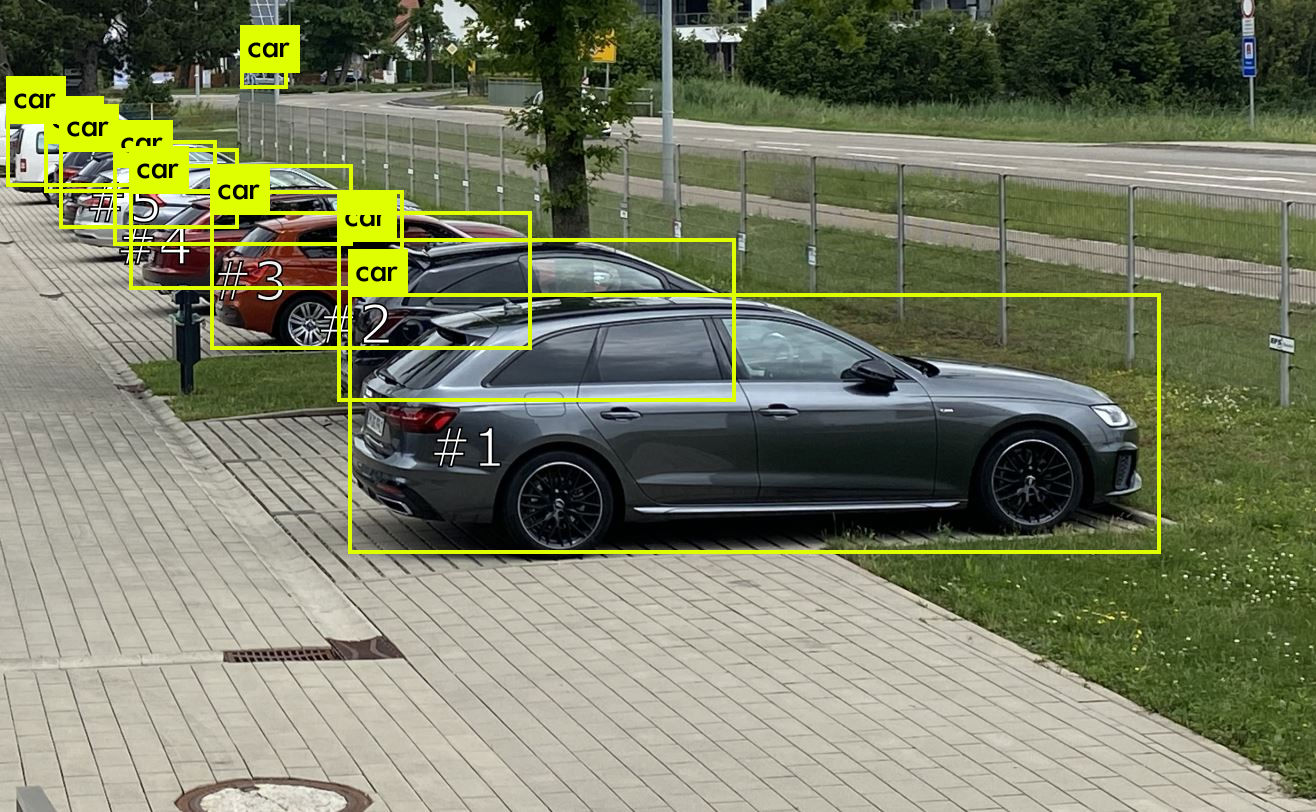
\includegraphics[scale=0.3]{imagens/predictions.jpg}
\caption{Output image with boundary boxes predictions}
\label{fig:park_predict}
\end{figure}



\begin{table}[H]
\centering
\caption{Accuracy of the proposed framework in object detector and classification}
\begin{tabular}{c|c}
\hline
Predicted Label & Accuracy \\ \hline
Car             & 91\%     \\ \hline
Car             & 31\%     \\ \hline
Car             & 96\%     \\ \hline
Car             & 94\%     \\ \hline
Car             & 95\%     \\ \hline
Car             & 98\%     \\ \hline
Car             & 47\%     \\ \hline
Car             & 97\%     \\ \hline
Car             & 98\%     \\ \hline
\end{tabular}
\label{tab:accuracy}
\end{table}



Figure \ref{fig:framework_predict} is shown the frontend of the application of this work. It was developed using Python and Javascript to allow the browser to communicate with the model. The Python module is composed of the libraries called sockets, and it permits the communication over many cameras and shares the stream information between the cameras and the command center. It was possible because the cameras used in the tests have an internal wireless network. Based on it, a script with a proxy function was developed to take care of this behavior. 

The backend side of this project is described in Appendix \ref{ap:app}, where there is information about the pre-processing step, training step, object detection, and the frontend scenario as well. The network was built using the framework Pytorch \cite{paszke2019pytorch}. This script permits the Darknet abstraction to perform object detection and object recognition, and with all of this information, the step to predict the distance was combined to show the output. 

The camera 1 of the Figure \ref{fig:framework_predict} is used only to perform the boundary boxes detection, and camera two is used to perform the distance prediction. This solution was embedded in a module to work as a controller of this framework.

The experiments also led us to measure the multi-cameras method's rapidity by computing the number of frames treated per second. The average of frames per second through all the experiments is 45.57 frames per second, enough for real-time treatments. 

\begin{figure}[H]
\centering
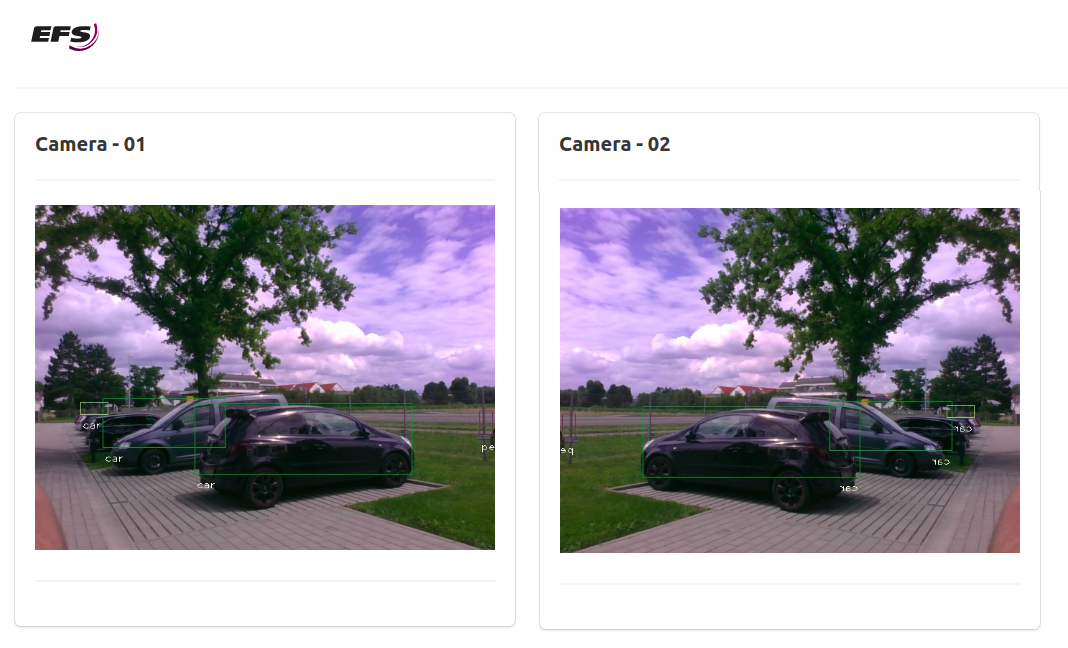
\includegraphics[scale=0.8]{imagens/output_framework.png}
\caption{Output image with predictions }
\label{fig:framework_predict}
\end{figure}



\section{Validation and Comparison between the Approaches}

For validation purpose, it was used a commercial laser measurement as shown in Figure \ref{fig:laser_meas}, this model is known as Bosch DLE 40 Professional {\tiny{\textregistered}}. 



\begin{figure}[H]
\centering
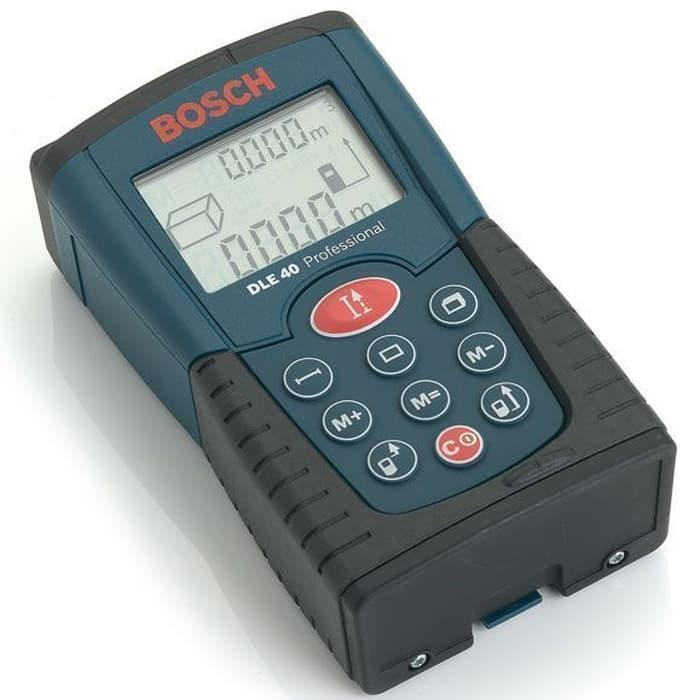
\includegraphics[scale=0.3]{imagens/trena.jpg}
\caption{Commercial laser measurer}
\label{fig:laser_meas}
\end{figure}

The current error rate is $ \pm 1.5 mm $, we repeated the measure three times and computed the mean and standard deviation. In Table \ref{tab:tab_measure} is shown the measurements with the camera positioned at $2.01$ m from the ground. Figure \ref{fig:park} is established the position of the cars along the parking lot. The reason to measure three times is that the manual is written on sunny days and can bias the measurement. 



\begin{table}[H]
\centering
\caption{Measurements collected with a commercial measurer}
\begin{tabular}{l|l|l|l|l} 
\toprule
Car & First measure (m) & Second measure (m) & Third measure (m) & Mean (m) \\
\#1   & 4.25          & 4.47           & 4.51           & 4.41 \\
\#2   & 11.01         & 11.21          & 11.11          & 11.11\\
\#3   & 16.12         & 16.35          & 16.26          & 16.24\\
\#4   & 19.63         & 19.69          & 19.66          & 19.66\\
\#5   & 23.08         & 23.18          & 23.01          & 23.09\\
\bottomrule
\end{tabular}
\label{tab:tab_measure}
\end{table} 


To compare the differences between the approaches and the real distance computed with the tool from Figure \ref{fig:laser_meas}. Table \ref{tab:total} was built to facilitate the visualization of these outputs. 


\begin{table}[H]
\centering
\caption{Comparison between the algorithms and real data}
\begin{tabular}{l|l|l|l|l} 
\toprule
Car & Camera Calibration (m) & Known Map (m) & Multicameras (m) & Real distance (m) \\
\#1   & 4.05          & 4.43           & \textbf{4.40 }          & 4.41 \\
\#2   & 10.67         & 10.98          & \textbf{11.05 }         & 11.11\\
\#3   & 15.52         & \textbf{16.01}          &\textbf{ 16.01 }         & 16.24\\
\#4   & \textbf{19.55}         & 18.99          & 19.92          & 19.66\\
\#5   & 20.08         & 22.18          & \textbf{24.08}          & 23.09\\
\bottomrule
\end{tabular}
\label{tab:total}
\end{table} 

It is necessary to examine the error between the real value. For this, a Python script was implement using Pandas Library \cite{mckinney2011pandas} to take care of the collected data. The error analysis was implemented to make it easier for the visualization of the best-applied technique. 

The pre-processed samples are used as input for the algorithms under text, resulting in estimations of the true position value. Results are expressed in terms of the RMSE, given by (\ref{eq:rmse}):
%
\begin{equation} \label{eq:rmse}
\text{RMSE}(f, \hat{f}) = \sqrt{\frac{1}{n_\text{samples}} \sum_{i=0}^{n_\text{samples} - 1} (f_i - \hat{f}_i)^2},
\end{equation}
%
calculated for each estimator $\hat{f}_i$, referenced either from the measurement tool of Figure \ref{fig:laser_meas} true value $f_i$ as read at the end of each measurement.

Figure \ref{fig:rmse} is shown a chart with the three proposed techniques using (\ref{eq:rmse}), where it is possible to see in specific points the multi-cameras approach was better than camera calibration.

\begin{figure}[H]
\centering
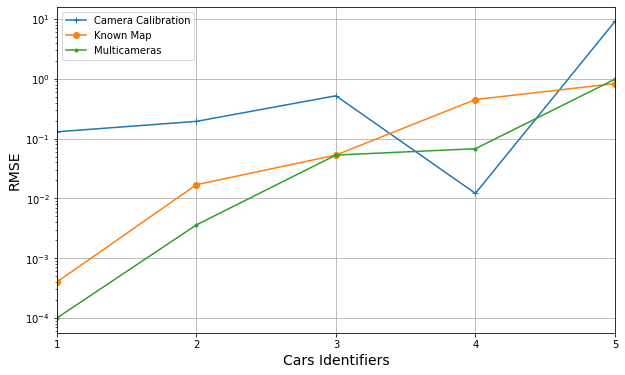
\includegraphics[scale=0.6]{imagens/plot.png}
\caption{RMSE of estimated estimate position for each algorithm for different detected car, referenced to values measured by the commercial laser measurer}
\label{fig:rmse}
\end{figure}